\chapter{Mechanical Design}

\graphicspath{{./Figures/Mechanical Design/}}
%	\item Outline the purpose and scope of the chapter.
 Modeling In this chapter, the details of the mechanical design are presented.
 where it goes from the initial conceptual design to the final design showing in the process the design decision-making for each critical point, This chapter emphasis the detailed description of the precise placement and alignment of different components such as the motors, wheels, battery, boards, and others to maintain the seamless integration of all the components into the robot body.
%	\item Briefly describe the mechanical design's role in the overall project.
\newline
The mechanical design serves as an important pillar to define the new physical form, size, and shape of the TWIPR. Depending on how these criteria are defined, the robot would interact with the environment.
taking into account that the design directly influences the center of gravity, which is crucial to consider in our robot due to the inverted pendulum nature to be able to balance and maintain the upright position.
In addition to the impact that the design has on the maneuverability of the robot and how it would respond to the control signals to be able to execute a task.
\newpage
\section{Design Objectives and Requirements}

%	Detail the primary objectives of the mechanical design
	The main objective is to come up with a new design for a multiple joints Robot to perform complex dynamic movements.
	This robot would be based on the Two wheeled inverted pendulum robots.
	The new design would add more degrees of freedom to enable the more complex movements.
	This enhances the robot's capabilities where it can execute more diverse scenarios.
%	\item List the requirements that the design must meet (e.g., weight limits, size constraints, mobility requirements).
	Initially, the main requirement was to add two more degrees of freedom where originally it used to have one degree of freedom in the wheels.
	The new design has three degrees of freedom, one in the wheels, one as a knee joint and one as a hip joint.
	The current design has two identical legs.

\section{Conceptual Design}
%Discuss the initial design concepts.
As for the initial design concepts the body was that main point of focus as shown in the figure \ref{fig:initialdesigns}.Three initial designs where considered mainly for the body.\ Symmetrical vertical body in figure A, symmetrical horizontal body in figure B and leaning forward body in figure C\@.
\ For the three designs, two independent legs where considered.
two designs where considered for the legs, the normal joint leg and the compliant leg

\begin{figure}[h]
	\centering
	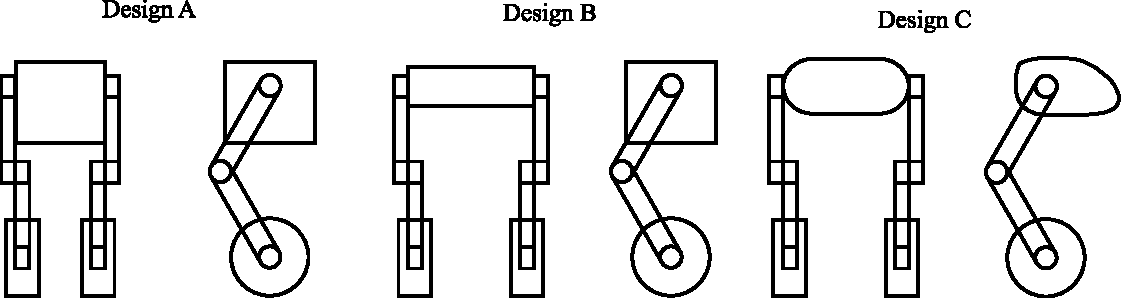
\includegraphics[width=1\linewidth]{Conceptual Design}
	%\includegraphics[width=0.5\linewidth]{Figures/Mechanical Design/Conceptual_Design}
	\caption[Initial Design Concepts]{Three initial Design Concepts for the robot body}
	\label{fig:initialdesigns}
\end{figure}
Two main designs where considered for the legs, the normal joint leg and the compliant leg.
The compliant leg is more flexible and can be used to absorb the shock from the ground.\ The normal joint leg is more rigid and can be used to generate more torque.in addition, the normal is more relative to our use-case as it can precisely control the position of the leg.
% figure for the leg designs concepts
\begin{figure}[h]
	\centering
	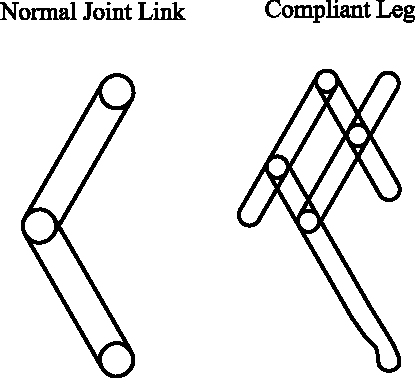
\includegraphics[width=0.4\linewidth]{Leg Design}
	\caption[Leg Design Concepts]{Leg Design Concepts}
	\label{fig:legdesignsjbhi}
\end{figure}

%Explain the decision-making process for selecting the final concept.
% Include sketches or early design models.
\section{Schmatic Representation of the Robot}
% the schematic representation of the robot should show the location of the different components such as the motors, wheels, battery, boards, and others
%figure for the schematic representation of the robot

\section{Initial Calculations}
%figure for the initial calculations
\begin{figure}[h]
	\centering
	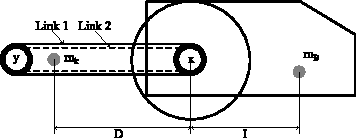
\includegraphics[width=0.7\linewidth]{Initial Calculations}
	\caption[Initial Calculations]{Initial Calculations}
	\label{fig:initialcalculations}
\end{figure}
One of the main critical positions for the robot, as shown in the figure \ref{fig:initialcalculations} is the position where the center of mass of the body and the center of mass of the legs are the furthest away from point x on the horizontal axis.It is important to make the initial torque calculations to be able to select the right motors for the robot.
Starting from that position first, the robot should be able to balance itself and maintain the upright position.
secondly, the robot should be able to change the knee angle to lift the body while maintaining its balance.
The calculations are based on some assumptions and simplifications, Considering only half the body weight and one leg.
As shown in the figure, The Wheel motor shaft is aligned with the hip joint, the minimum torque required to balance the robot is calculated as follows:

The summation of the torques around point x should be equal to zero to maintain the balance with minimum motor torque.
\begin{equation}
	\sum_{i=1}^{n} \tau_{i}=0
\end{equation}
\begin{equation}
	\sum_{i=1}^{n} \tau_{i}=m_{B}*g*D-m_{K}*g*I
\end{equation}
\begin{equation}
	\sum_{i=1}^{n} \tau_{i}=0.5*9.81*0.03-0.2*9.81*0.5*0.15=0 Nm
\end{equation}
The Lengths of D and I can be modified to make sure that the summation of the torques around point x is equal or approximately equal to zero.
This will make sure that the robot can balance itself with minimum wheel motor torque.
The torques can cancel each other out by readjusting the lengths of D or I and also by modefiing the weight distribution in the body and the legs.

The torque required to lift the body is calculated as follows:
\begin{equation}
	\sum_{i=1}^{n} \tau_{i}=m_{B}*g*(D+I)-m_{K}*g*L_{1}
\end{equation}
\begin{equation}
	\sum_{i=1}^{n} \tau_{i}=0.5*9.81*(0.03+0.15)-0.1*9.81*0.5*0.15=0.9555 Nm
\end{equation}
0.9555 Nm is the minimum torque required to hold the body in position.
The Knee motor should be able to generate more torque to be able to lift the body and change the knee angle.

\begin{table}[h]
	\centering
	\caption{Initial Calculations Assumptions}
	\label{tab:initialcalculationsassumptions}
	\begin{tabular}{lcl}
		\toprule
		Parameter & Value & Description 			  \\
		\midrule
		$m_B$         & 0.5 kg  & Mass of the body  \\
		$m_K$         & 0.2 kg  & Mass of the Knee including the two legs\\
		$L_1$         & 0.15 m   & Length of Link 1  \\
		$L_2$         & 0.15 m   & Length of Link 2   \\
		$d$ 	  	  & 0.3 m   & distance from the hip joint axis to the center of mass of the body   \\
		\bottomrule
	\end{tabular}
\end{table}

\begin{notebox}
	\textbf{To reduce the needed torque to lift we can:}
	%bullit points
	\begin{itemize}
		\item Shorten the links
		\item Reduce the body weight
		\item Use gearbox to increase the torque
	\end{itemize}
\end{notebox}
\newpage
\section{Detailed Design Development}
% Elaborate on the development of the detailed mechanical design.
Throughout the design process, modularity and ease of assembly were considered.
The design was broken down into three main parts: the body, the hip-knee link, and the knee-wheel link.
Print iterations were made to ensure that the parts fit together and that the robot could be assembled with ease. Modifications were made to simplify the printing process and reduce the support material used.


\subsection{Body Design}
% Discuss the design of the body.
The body design is the main part of the robot, it is the main structure that holds all the components together.
The components that are mounted on the body are the hip motors, the battery, camera, sensor, a rack that includes the power distribution board, the microcontroller board attached to the Raspberry Pi.The optimization of the body design is crucial to be able to fit all the components in a compact form and at the same time distribute the weight equally to maintain the balance of the robot.
Different design features were considered, such as the cable management, the fastening features specifically designed to easily mount the battery, organize the cable between the boards and the rest of the robot parts.
%figure 1 for the body design
\begin{figure}[h]
	\centering
	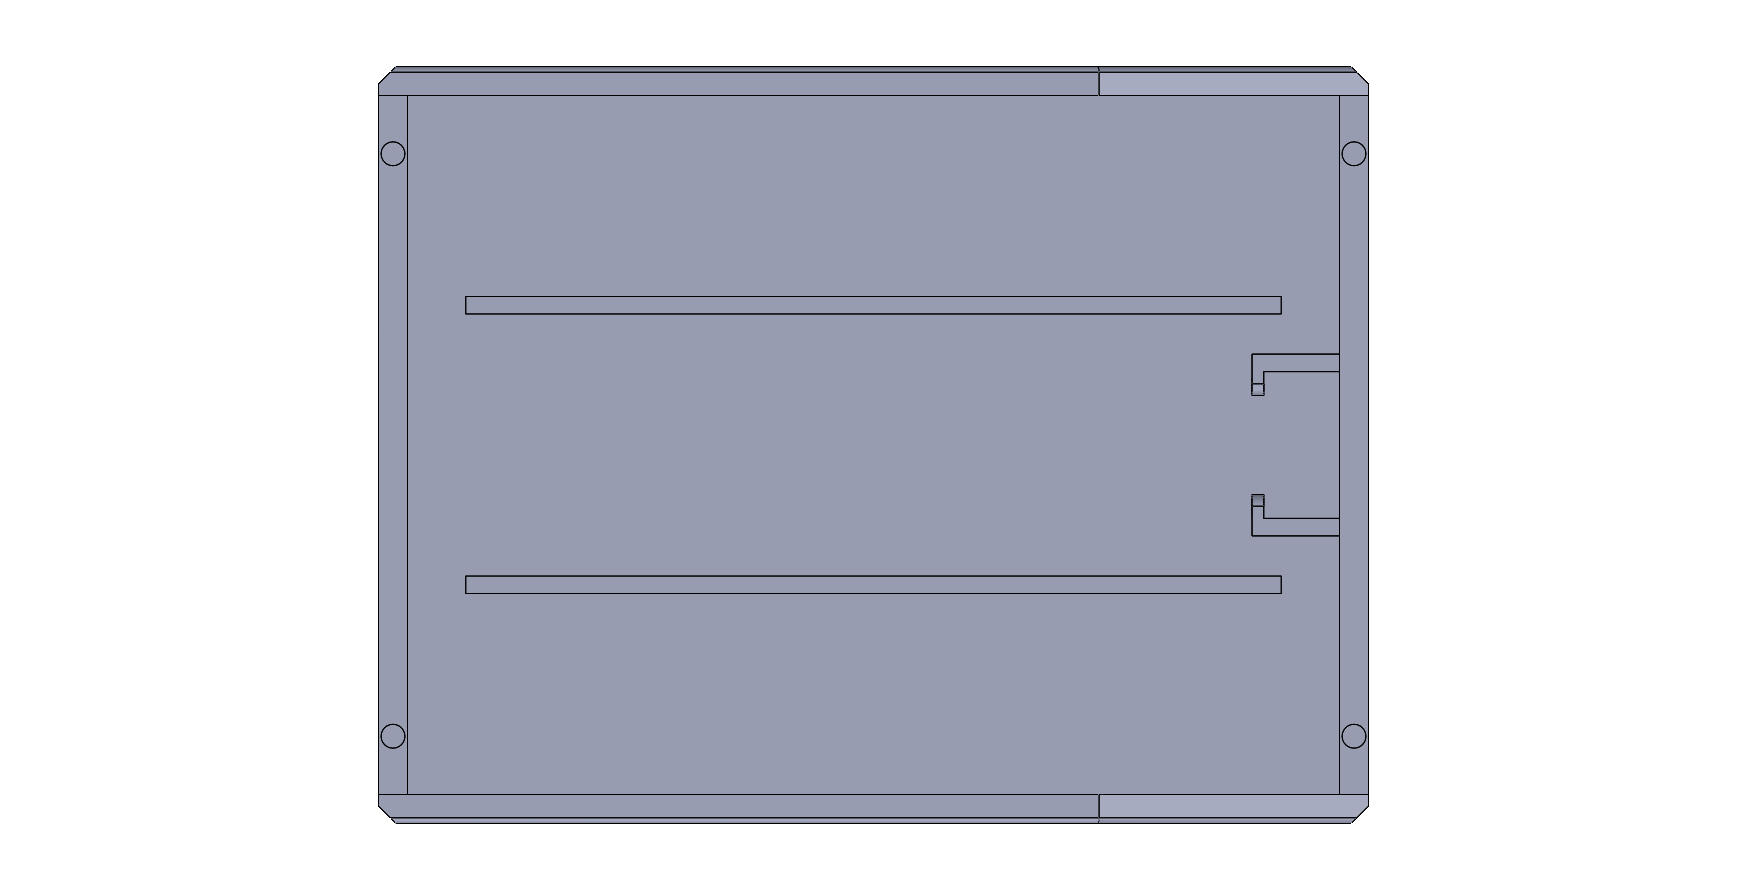
\includegraphics[width=1\linewidth]{Body_Design_1}
	\caption[TOP view of the Body Design]{TOP view of the Body Design}
	\label{fig:bodydesign1}
\end{figure}
%figure 2 for the body design
\begin{figure}[h]
	\centering
	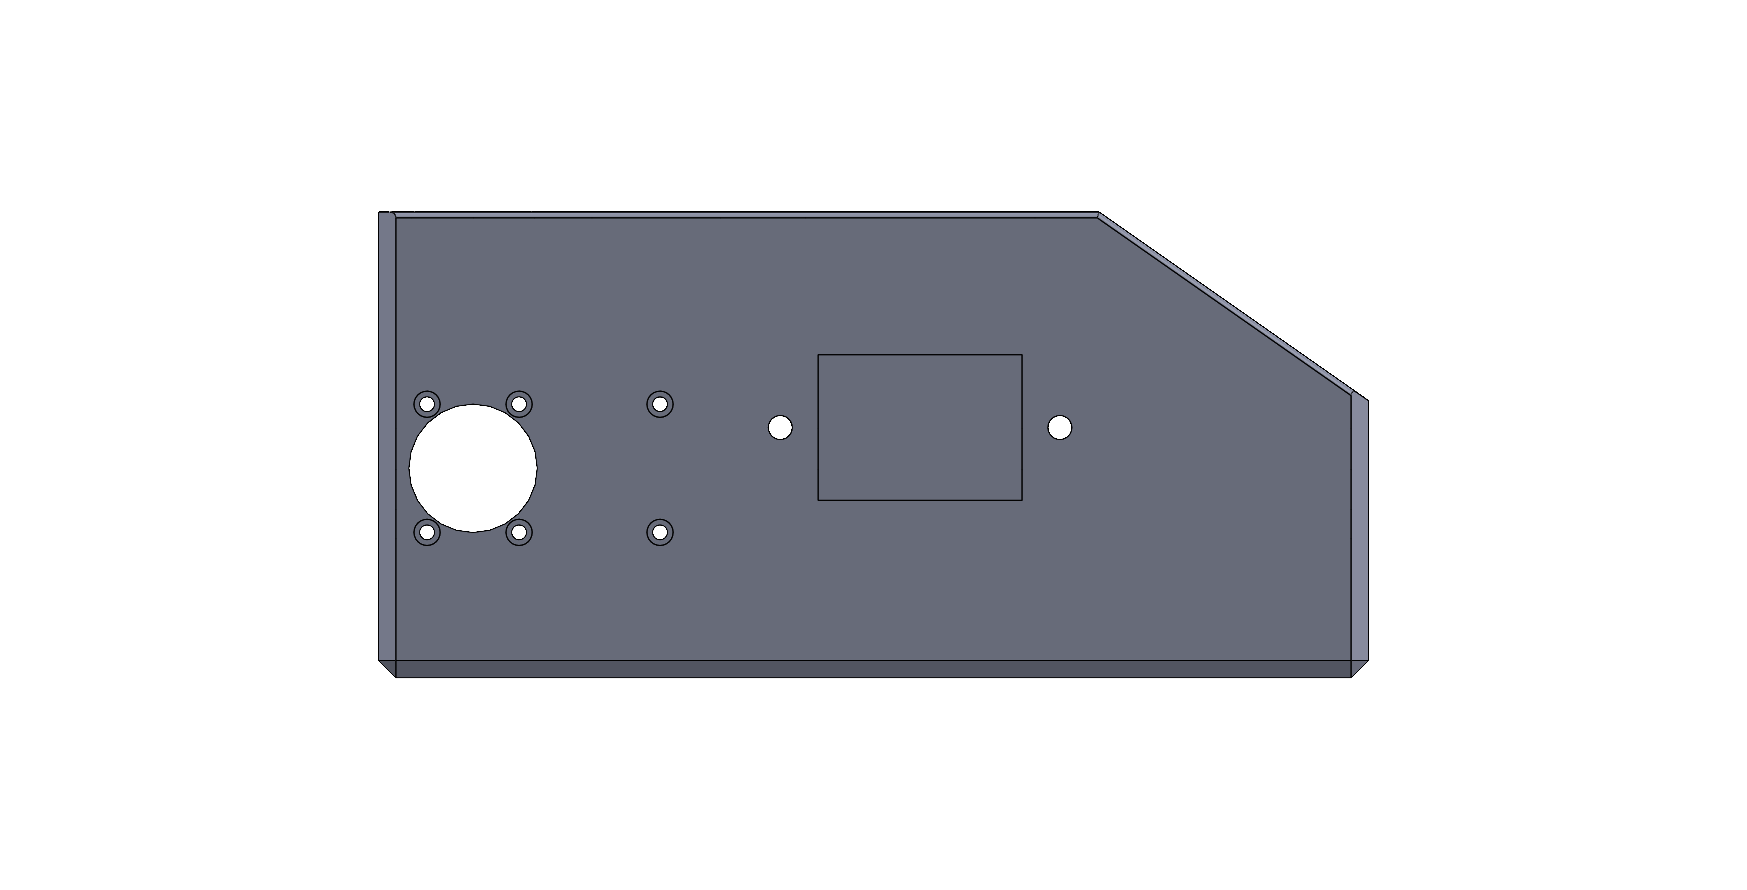
\includegraphics[width=1\linewidth]{Body_Design_2}
	\caption[Side view of the Body Design]{side view of the Body Design}
	\label{fig:bodydesign2}
\end{figure}
%figure 3 for the body design
\begin{figure}[h]
	\centering
	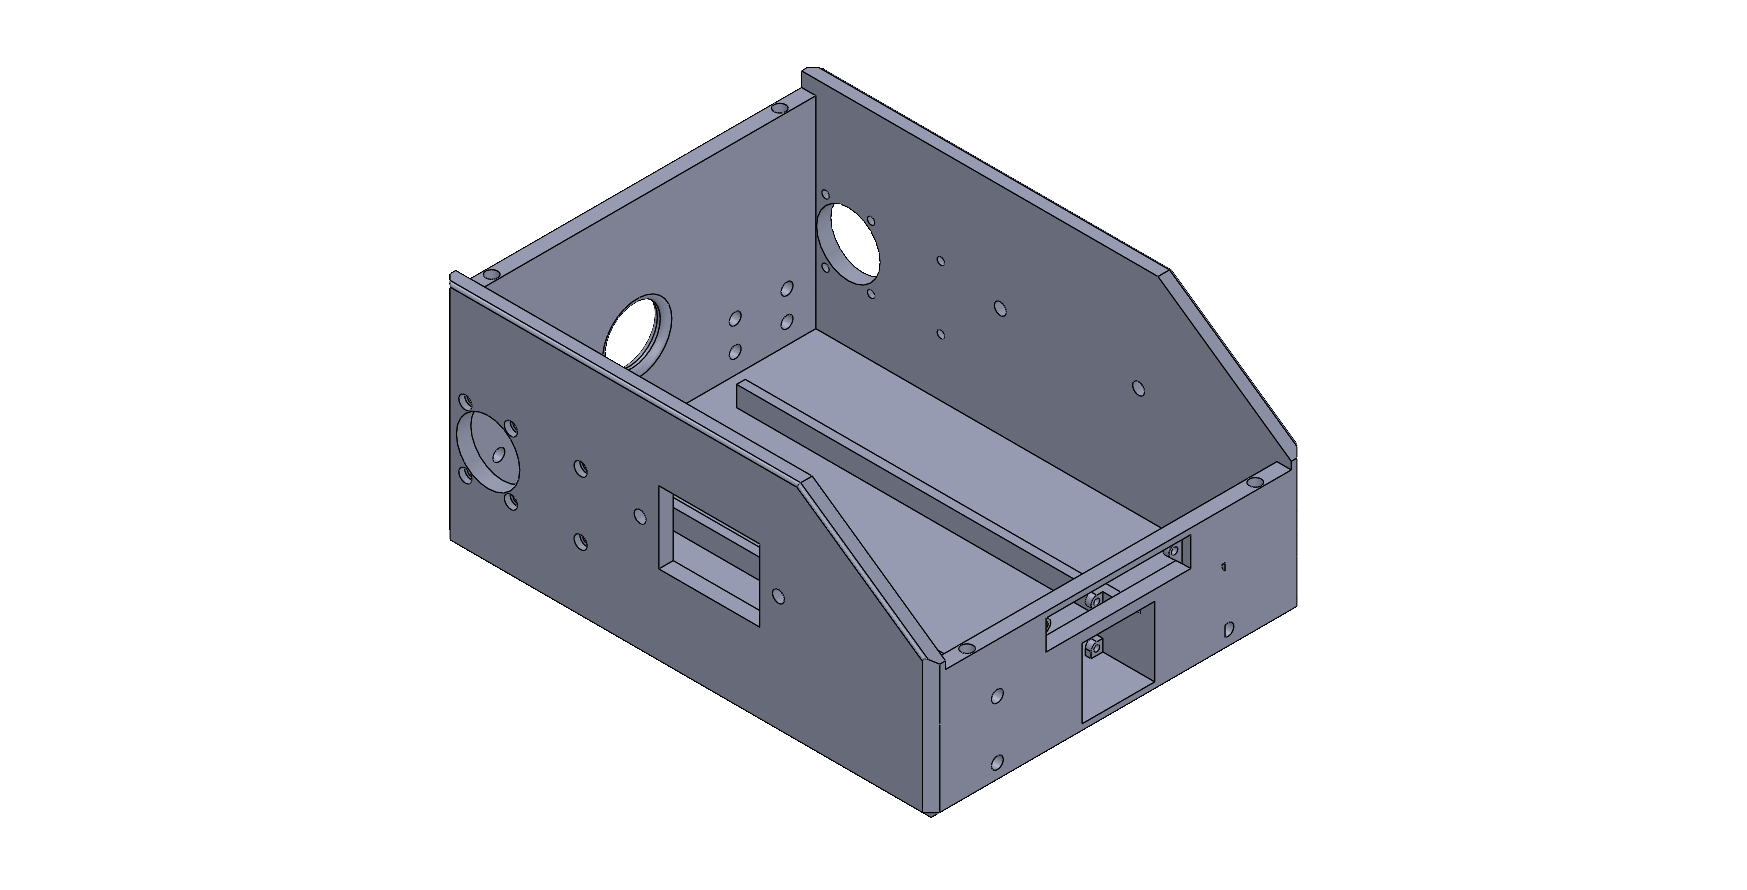
\includegraphics[width=0.8\linewidth]{Body_Design_3}
	\caption[3D view of the Body Design]{3D view of the Body Design}
	\label{fig:bodydesign3}
\end{figure}

\newpage
\subsection{Hip Knee Link Design}
% Discuss the design of the hip knee Link.
This link connects the hip body axis to the knee axis.
The design of this link includes the knee motor housing form one-side and a frame to attach to the output horn of the hip motor.
The motor housing is designed to ensure the fixed placement of the motor inside the link, As shown in the figure, \ref{fig:bodykneelink1} Cable management is also considered in the design of this link to make sure that the cables are not interfering with the movement of the link.The curvature of the link creates enough clearance so that when the hip axis is aligned with the wheel axis, they would not touch with each other even when considering the elastic bending of the legs.
%figure 1 for the Body_Knee_link
\begin{figure}[h]
	\centering
	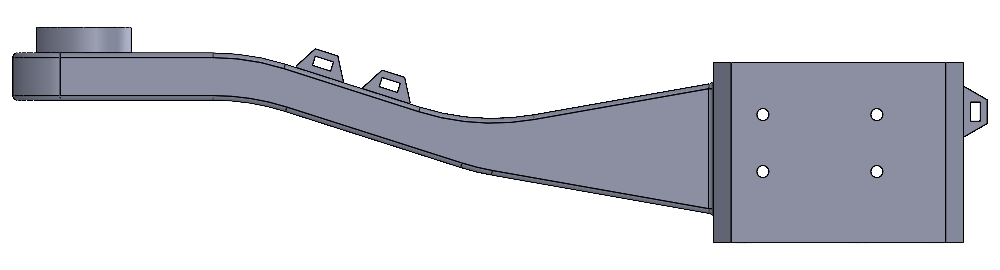
\includegraphics[width=1\linewidth]{Body_Knee_Link_1}
	\caption[TOP view of the Body Knee Link]{TOP view of the Body Knee Link}
	\label{fig:bodykneelink1}
\end{figure}
%figure 2 for the Body_Knee_link
\begin{figure}[h]
	\centering
	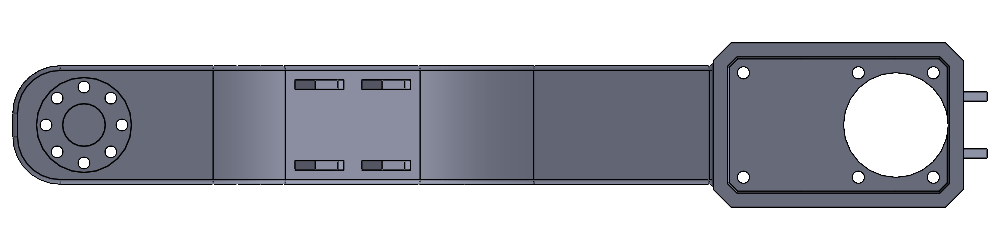
\includegraphics[width=1\linewidth]{Body_Knee_Link_2}
	\caption[Side view of the Body Knee Link]{side view of the Body Knee Link}
	\label{fig:bodykneelink2}
\end{figure}
%figure 3 for the Body_Knee_link
\begin{figure}[h]
	\centering
	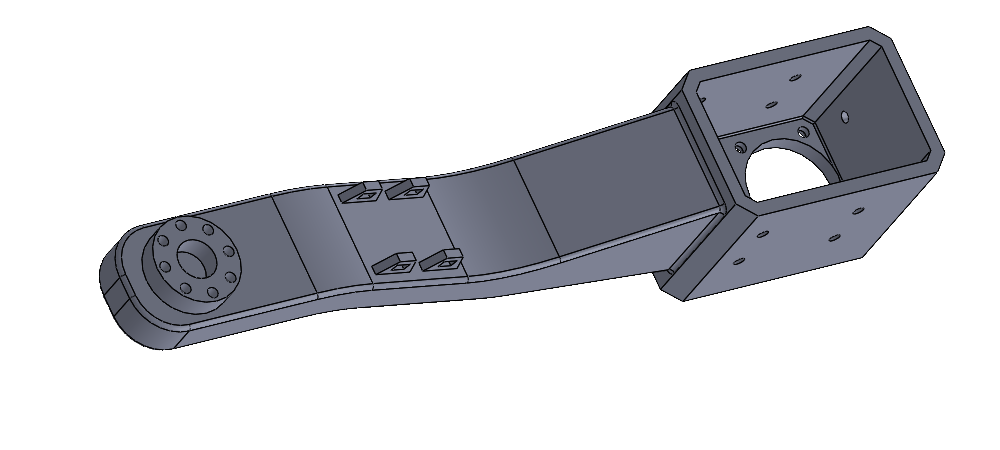
\includegraphics[width=1\linewidth]{Body_Knee_Link_3}
	\caption[3D view of the Body Knee Link]{3D view of the Body Knee Link}
	\label{fig:bodykneelink3}
\end{figure}


\subsection{Knee Wheel Link Design}
% Discuss the design of the Wheel_Knee_link.
This link connects the knee axis to the wheel axis. The design of this link includes the wheel motor mounting form one-side and a frame to attach to the output horn of the knee motor from the other side.
%figure 1 for the Wheel_Knee_link
\begin{figure}[h]
	\centering
	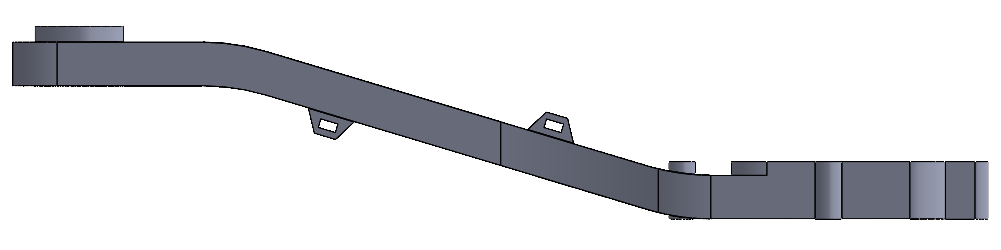
\includegraphics[width=1\linewidth]{Wheel_Knee_Link_1}
	\caption[SIDE view of the Knee Wheel Link]{SIDE view of the Knee Wheel Link}
	\label{fig:wheelkneelink1}
\end{figure}
%figure 2 for the Wheel_Knee_link
\begin{figure}[h]
	\centering
	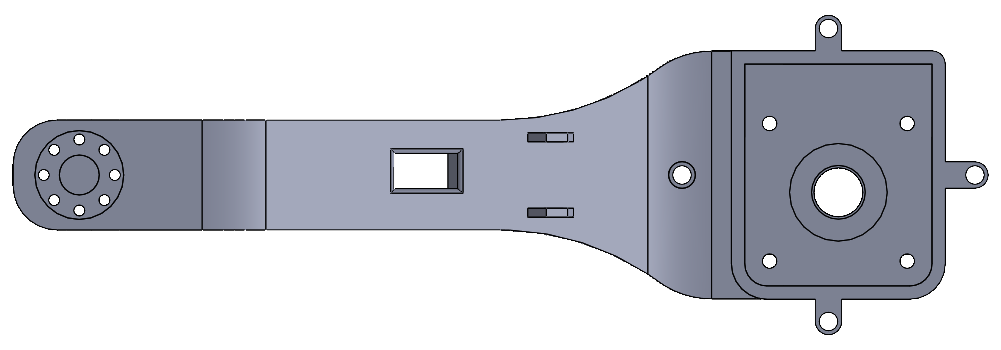
\includegraphics[width=1\linewidth]{Wheel_Knee_Link_2}
	\caption[TOP view of the Knee Wheel Link]{TOP view of the Knee Wheel Link}
	\label{fig:wheelkneelink2}
\end{figure}
%figure 3 for the Wheel_Knee_link
\begin{figure}[h]
	\centering
	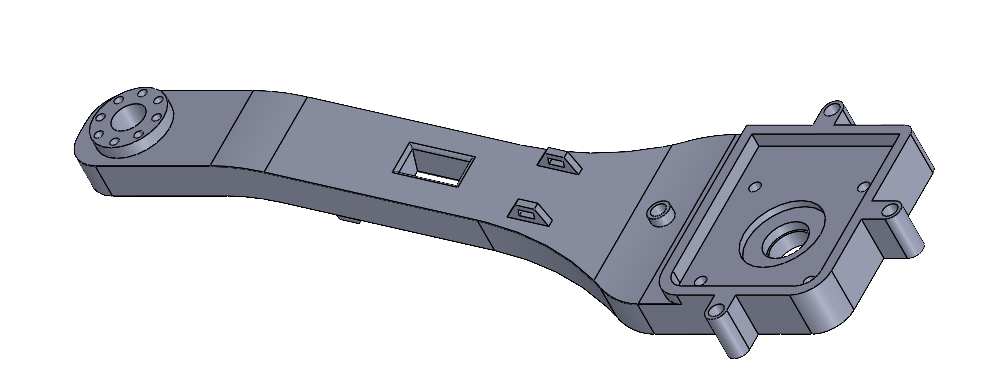
\includegraphics[width=1\linewidth]{Wheel_Knee_Link_3}
	\caption[3D view of the Knee Wheel Link]{3D view of the Knee Wheel Link}
	\label{fig:wheelkneelink3}
\end{figure}

\subsection{Full Design}


%figure 1 for the Robot_Assembly
\begin{figure}[h]
	\centering
	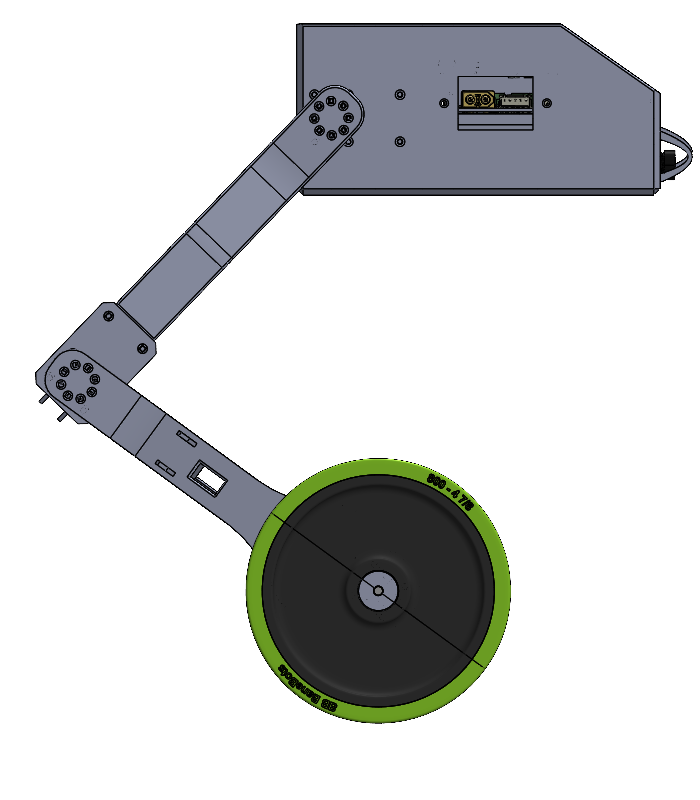
\includegraphics[width=1\linewidth]{Robot_Assembly_1}
	\caption[Side view of the Robot Assembly]{Side view of the Robot Assembly}
	\label{fig:robotassembly1}
\end{figure}
%figure 2 for the Robot_Assembly
\begin{figure}[h]
	\centering
	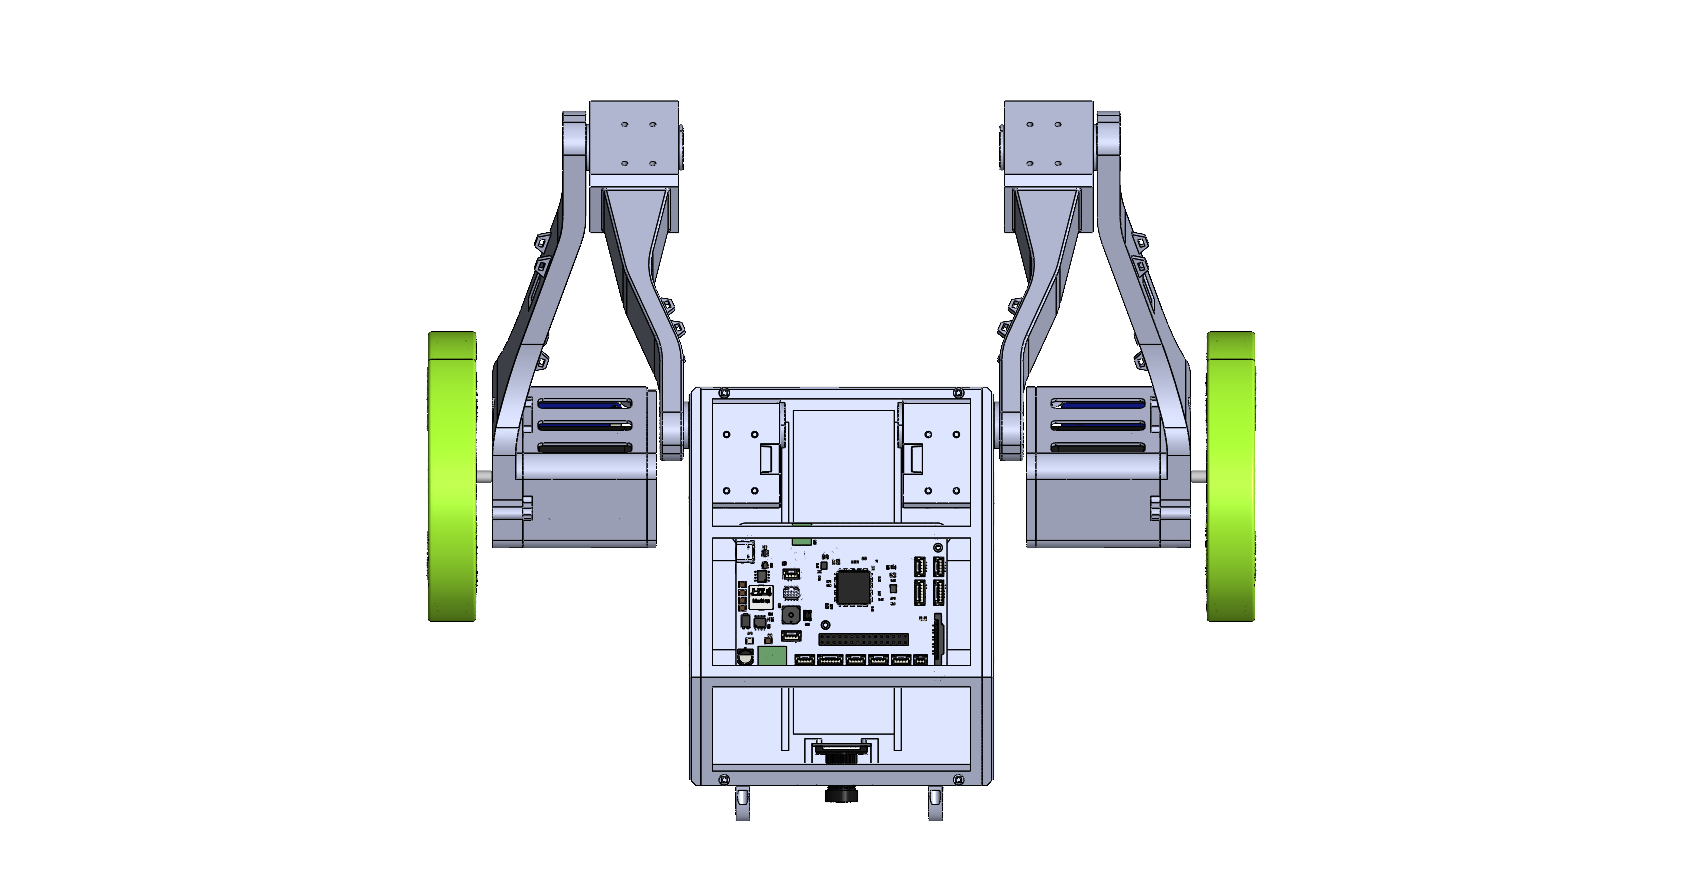
\includegraphics[width=1\linewidth]{Robot_Assembly_2}
	\caption[Front view of the Robot Assembly]{Front view of the Robot Assembly}
	\label{fig:robotassembly2}
\end{figure}
%figure 3 for the Robot_Assembly
\begin{figure}[h]
	\centering
	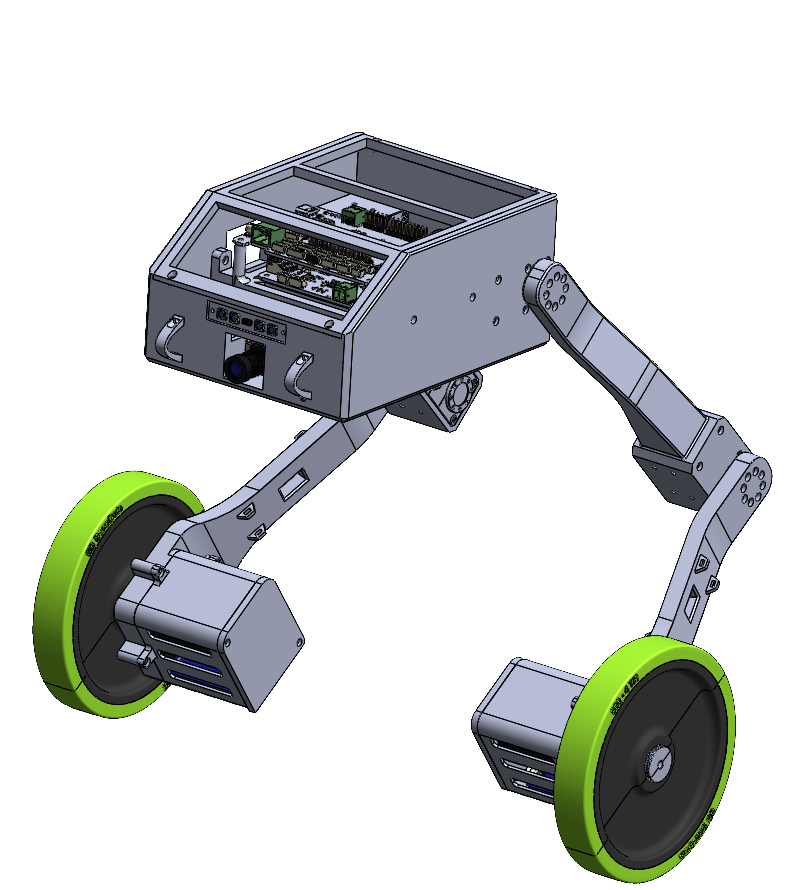
\includegraphics[width=1\linewidth]{Robot_Assembly_3}
	\caption[3D view of the Robot Assembly]{3D view of the Robot Assembly}
	\label{fig:robotassembly3}
\end{figure}
\subsection{Boards Mounting rack}
\subsection{Safety considerations}
% the motor cover, the face shield of the body and the body cover
Safety is a crucial aspect to consider in the design of the robot. The robot is designed to be safe to operate in the environment and safe to interact with humans. Clearences are considered in the design to make sure that moving parts wouldn't interfere with eachother.
The motor cover is designed to protect the motor from any external objects that might interfere with the motor operation.
%Two subfigures side by side of the motor cover

The face shield of the body is designed to protect the components inside the body from any external objects that might hit the robot.
%two subfigures side by side of the face shield



\section{Design for Manufacturability and Assembly}
% Discuss how the design facilitates manufacturing and assembly.
% Explain any design choices made to simplify these processes of manufacturing and assembly.
\section{Prototyping and Iterative Design}
% Discuss the process of prototyping.
% Explain how feedback from prototyping phases was incorporated into design revisions.


